\documentclass{mnnit}

\usepackage{graphicx}
\usepackage{booktabs}
\usepackage{amsmath}
\usepackage{array}
\usepackage{url}
\usepackage{etoolbox}
% Single spacing inside figures and tables (the class used to do this; see mnnit.cls).
\AtBeginEnvironment{figure}{\def\baselinestretch{1}\normalsize}
\AtBeginEnvironment{table}{\def\baselinestretch{1}}

\graphicspath{{figures/}}
\setlength{\emergencystretch}{2.5em}

% ---------------------------------------------------------------------------
% Group-project front matter. mnnit.cls writes the undertaking in the first
% person singular and puts \@author inside a sentence, so both pages are
% redefined here for four authors.
% ---------------------------------------------------------------------------
\newcommand{\authorsinline}{Shaurya Pratap Singh (20233262), Surya Pratap Singh (20233283), Vishesh Vigh (20233583), and Sehar Majid Abdi (20233561)}

\makeatletter
\def\undertakingpage{\newpage%
    \renewcommand{\baselinestretch}{1.3}
    \vspace*{\fill}
    \centerline{\LARGE\bf UNDERTAKING}
    \vspace{2cm}
    \begin{center}
    \begin{minipage}{5.2in}
    \parindent=0pt
    We declare that the work presented in this report titled
    ``{\sl\@title}'', submitted to the \mbox{\@dept} Department, \@college, for
    the award of the {\bf\emph{\@degree}} degree in \mbox{\bf\emph{\@specialization}},
    is our original work. We have not plagiarized or submitted the same work for
    the award of any other degree. In case this undertaking is found incorrect, we accept
    that our degree may be unconditionally withdrawn.\par
    \vspace*{1.5cm}
    \@submitdate\\Prayagraj\par
    \vspace*{1.8cm}
    \begin{tabular}{@{}p{2.5in}p{2.5in}@{}}
    \rule{2.1in}{0.4pt} & \rule{2.1in}{0.4pt}\\
    Shaurya Pratap Singh (20233262) & Surya Pratap Singh (20233283)\\[1.6cm]
    \rule{2.1in}{0.4pt} & \rule{2.1in}{0.4pt}\\
    Vishesh Vigh (20233583) & Sehar Majid Abdi (20233561)
    \end{tabular}
    \end{minipage}
    \end{center}
    \vspace*{\fill}
}

\long\def\signature#1{%
\begin{center}
\begin{minipage}{5.2in}
\parindent=0pt
Certified that the work contained in the report titled
``{\sl\@title}'', by \authorsinline, has been carried out under my
supervision and that this work has not been submitted elsewhere for a
degree.
\par
\vspace{3cm}
\hbox to 5.2in{\@submitdate\hfill
    \vbox{\hsize 3in\vrule width 2in height0.4pt\par#1}\hss}
\end{minipage}
\end{center}
}
\makeatother

% Citations. The class redefines thebibliography after loading natbib, which
% leaves \cite unresolved (the template's own PDF prints "?"). References are
% therefore a numbered list cited with \rc{key}, which needs no BibTeX run.
\makeatletter
\newcommand{\rc}[1]{[\def\rc@sep{}\@for\rc@key:=#1\do{\rc@sep\ref{ref:\rc@key}\def\rc@sep{, }}]}
\makeatother


% Single-spaced contents page with a compact heading, so it fits on one page.
\let\oldtableofcontents\tableofcontents
\makeatletter
\renewcommand{\tableofcontents}{\begingroup\renewcommand{\baselinestretch}{1.0}\normalsize
  \def\@makeschapterhead##1{{\parindent\z@\raggedright\normalfont\Huge\bfseries ##1\par\nobreak\vskip 20\p@}}%
  \oldtableofcontents\endgroup}
\makeatother

\begin{document}
\title{Neuro-Symbolic Reasoning over Patient-Specific Knowledge Graphs for Breast Cancer Progression Prediction}
\author{\begin{tabular}{ll}
Shaurya Pratap Singh & (20233262)\\
Surya Pratap Singh & (20233283)\\
Vishesh Vigh & (20233583)\\
Sehar Majid Abdi & (20233561)
\end{tabular}}
\supervisor{Dr. Shashwati Banerjea}
\specialization{Computer Science \& Engineering}

\beforepreface

\prefacesection{Abstract}
Predicting whether and when a breast cancer will progress after treatment is a central question in oncology, and a
prediction helps a clinician only if it comes with reasons. We build a knowledge graph for each of the 1,083 breast
cancer patients of the TCGA PanCancer Atlas 2018 cohort. It links the patient to their tumour and to their altered genes,
and we join those genes to PrimeKG, a public biomedical knowledge graph of pathways, drugs, and diseases.

Graph neural networks (GNNs) trained on these graphs reach a concordance index (C-index) of about 0.62, and every model
family we tried stops near 0.67. We therefore turned the project towards explanation. A survival GNN supplies neural
evidence. For the symbolic side we replaced crisp IF--THEN rules with learned logic. We compared four survival-aware
reasoners: a Markov logic network whose formula weights are learned from survival times, probabilistic soft logic,
rules written by a reinforcement-learning agent, and a hybrid in which reinforcement learning proposes the Markov logic
formulas. The hybrid is our rule engine. Each explanation path is scored as $0.6\times$ neural $+\ 0.4\times$ rule.

The logic engine matches RuleKit's accuracy (C-index 0.63 against 0.62). 69\% of its weighted formulas reason over
knowledge-graph relations, against 10\% of RuleKit's rules. The fused model is statistically tied with the best
clinical model (0.664 against 0.675). Its month-of-progression estimate is within a year for 48\% of progressors. The
system writes an explained PDF report for every patient, grouped by when they progressed.

\prefacesection{Acknowledgements}
We thank our supervisor, Dr.\ Shashwati Banerjea, for guidance and for steering the project from raw accuracy
towards neuro-symbolic reasoning and interpretable patient reports. We thank the Department of Computer Science and
Engineering, MNNIT Allahabad, for its support. We are grateful to the TCGA Research Network and cBioPortal for the data,
to the Zitnik Lab for PrimeKG, and to the developers of PyTorch Geometric, lifelines, scikit-survival, and RuleKit.

\afterpreface

% ===========================================================================
\chapter{Introduction and Background}
% ===========================================================================

Breast cancer is the most commonly diagnosed cancer worldwide \rc{globocan}. After treatment, some patients never
relapse, some progress within months, and some progress after a decade. Clinicians estimate this risk mainly from
stage, lymph-node status, and molecular subtype \rc{pam50}. Tumour sequencing adds hundreds of gene alterations per
patient, but most of them mean little on their own.

A biomedical knowledge graph can put those alterations in context. PrimeKG \rc{primekg} connects genes to the pathways
they act in, the drugs that target them, and the diseases they are linked to. If a patient's altered gene sits in a
growth-signalling pathway, the graph can say so explicitly.

\section{Motivation}
A risk score without reasons is hard to trust in a clinic. Neural networks learn well from data but do not explain
themselves. Rules are readable but cannot weigh thousands of interacting facts. Neuro-symbolic AI
\rc{neurosymbolic} combines the two: a neural part learns from the data, and a symbolic part states its reasoning as
explicit, checkable knowledge. Our project began as a GNN benchmark. When accuracy saturated, we followed our
supervisor's direction and built a neuro-symbolic layer whose output is a readable report for every patient.

\section{Problem Statement}
Given a patient's clinical record, tumour mutations, and copy-number changes, together with PrimeKG, the system must
(i) estimate the risk of progression, (ii) estimate the month of progression when it happens, (iii) explain the
estimate with knowledge-graph paths and logic formulas, and (iv) present it as a clinical report grouped by
progression time. Outcome data must never leak into the inputs. Every reported prediction must come from a model that
did not see that patient during training.

\section{Contributions and Novelty}
\begin{enumerate}
  \item A leakage-checked pipeline from raw TCGA tables to patient graphs fused with PrimeKG, with 58 unit tests.
  \item A benchmark of seven GNN architectures and three training objectives, all evaluated out-of-fold.
  \item \textbf{Learned logic instead of IF--THEN rules.} We tried all three of our supervisor's suggestions (Markov
        logic, probabilistic soft logic, and reinforcement learning) as survival reasoners over 422 first-order facts.
        The chosen engine is new in two ways:
        \begin{itemize}
          \item it is a \emph{survival} Markov logic network, whose formula weights are learned with the Cox
                likelihood, so patients who have not relapsed yet are handled correctly;
          \item its formulas, many of them multi-step knowledge-graph chains, are \emph{proposed by a
                reinforcement-learning agent} that is rewarded only for rules that hold up on unseen patients.
        \end{itemize}
  \item Explanation paths scored as $0.6\times$ neural importance $+\ 0.4\times$ the weight of the formulas they
        support, with a top-$K$ cutoff.
  \item 1,083 patient reports in five progression groups, and two executed notebooks that document the work.
\end{enumerate}

\section{Background: Data and Knowledge Graph}
The Cancer Genome Atlas (TCGA) PanCancer Atlas profiled more than 10,000 tumours with uniform pipelines \rc{hoadley}.
We use its breast cancer cohort as distributed by cBioPortal \rc{cbioportal}. Its progression-free interval is the
recommended outcome for breast cancer \rc{tcgacdr}. PrimeKG \rc{primekg} merges 20 biomedical resources, including
Reactome pathways and DrugBank targets, into 129,375 nodes and over 8 million edges. Its genes keep their NCBI
Entrez identifiers, so patient genes can be matched exactly.

\section{Background: Graph Neural Networks}
A GNN updates every node from its neighbours' features. GCN \rc{gcn} averages neighbours, GraphSAGE \rc{graphsage}
keeps separate self and neighbour weights, attention models such as GATv2 \rc{gatv2} learn a weight per edge, and
R-GCN \rc{rgcn} learns one weight matrix per relation type. GNNExplainer \rc{gnnexplainer} finds which edges a trained
model relied on for a prediction, which gives every edge an importance score.

\section{Background: Survival Analysis}
Progression is a time-to-event outcome with \emph{censoring}: a patient with no recorded progression may still
progress after their last visit. The Kaplan--Meier curve \rc{km} estimates the share of patients still
progression-free over time, and the log-rank test \rc{logrank} compares two such curves. The Cox model \rc{cox} turns
patient features into a risk score and is fitted by the partial likelihood. Accelerated failure time (AFT) models
\rc{aft} predict the event time directly. Models are compared with the concordance index (C-index) \rc{harrell}: the
share of patient pairs in which the patient who progressed first received the higher risk. A C-index of 0.5 is a coin
flip and 1.0 is perfect.

\section{Background: Rules and Logic}
\textbf{Survival rules.} RuleKit's LR-Rules \rc{lrrules,rulekit} grows IF--THEN rules such as ``IF nodal stage is N0
AND age $\ge$ 41.5 THEN low risk'' by maximising the log-rank separation of the patients a rule covers. The rules are
crisp: a rule either fires or it does not, and it carries no weight.

\textbf{Markov logic networks (MLNs)} \rc{mln} attach a weight to each logic formula. A world that breaks a formula
with a large weight becomes less likely but is still possible. Learning an MLN means finding the formulas (structure
learning) and their weights.

\textbf{Probabilistic soft logic (PSL)} \rc{psl} allows truth values between 0 and 1 and turns each rule into a penalty
for how far it is from being satisfied. Inference is then a convex optimisation, which allows \emph{collective}
reasoning, for example letting similar patients influence each other.

\textbf{Reinforcement learning (RL) for rules.} A policy-gradient agent \rc{reinforce} learns from rewards rather than
labels. In knowledge-graph reasoning, agents have been trained to walk relation paths \rc{deeppath,minerva} and to
write logic rules \rc{rnnlogic}. We use RL to write survival rules.

% ===========================================================================
\chapter{Proposed Work}\label{ch:proposed}
% ===========================================================================

Figure~\ref{fig:pipeline} gives the overview. Patient graphs are built from TCGA and fused with PrimeKG. A survival
GNN and the logic reasoners run on the same patients and the same five folds. Their risks are combined in one Cox
model, and every patient gets a report that explains the prediction with knowledge-graph paths and logic formulas.

\begin{figure}[!htbp]
  \centering
  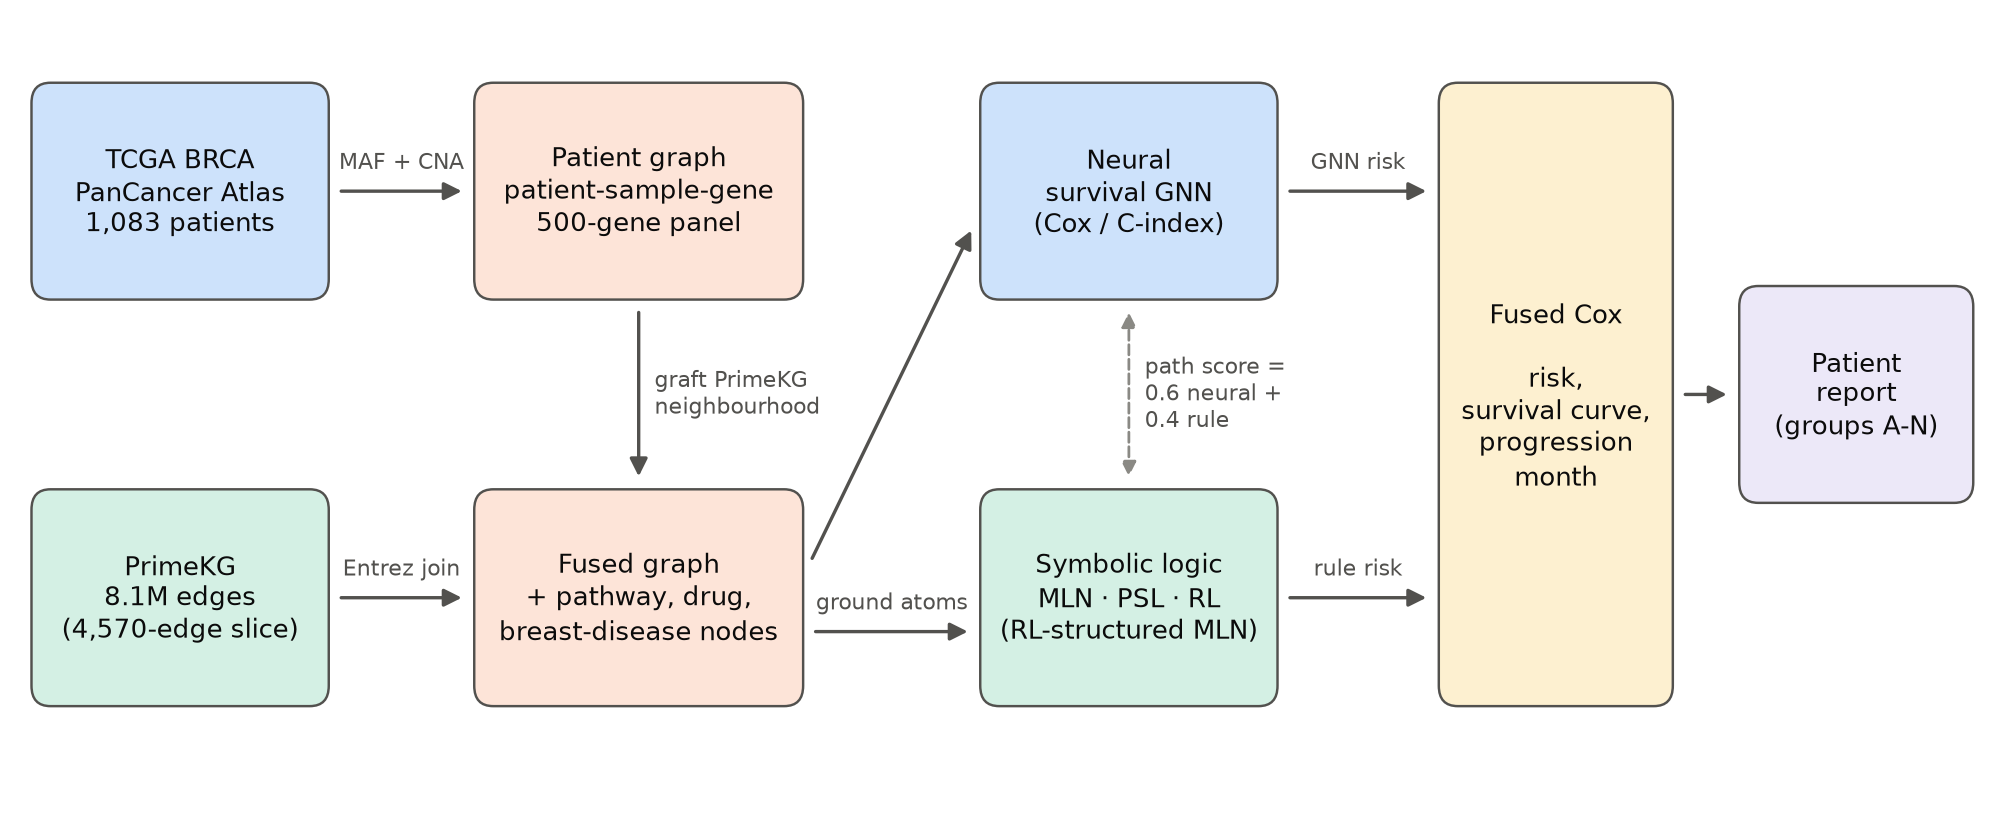
\includegraphics[width=0.75\textwidth]{fig_pipeline.png}
  \caption{Overview of the neuro-symbolic progression system.}
  \label{fig:pipeline}
\end{figure}

\section{Data and Labels}
We use the cBioPortal \texttt{brca\_tcga\_pan\_can\_atlas\_2018} study, checked against its official checksums: the
clinical tables, 126,252 mutation records, and copy-number calls for 25,128 genes. 1,083 patients have a usable
progression-free survival (PFS) record, and 145 of them progressed. Outcome columns (survival, progression, and
tumour-status fields) are blocked from every feature table by a guard function that the tests check.

The GNN benchmark uses a 36-month landmark label (498 patients, 89 events). The survival models and the reports use
the full follow-up time and event of all 1,083 patients.

\section{Patient Graphs and PrimeKG Fusion}
Each patient graph has the shape Patient $\rightarrow$ Sample $\rightarrow$ Gene. Genes are limited to a 500-gene
panel of the most frequently altered genes plus 27 known breast cancer drivers. PrimeKG's 8.1 million edges are
filtered once to 4,570 edges that touch the panel: protein--protein, gene--pathway, gene--drug, and gene--breast-disease
links. A patient's genes join PrimeKG on their Entrez identifiers, which adds each altered gene's partners, pathways,
drugs, and breast-disease links (Figure~\ref{fig:fused}). The median fused graph has 632 nodes.

\begin{figure}[!htbp]
  \centering
  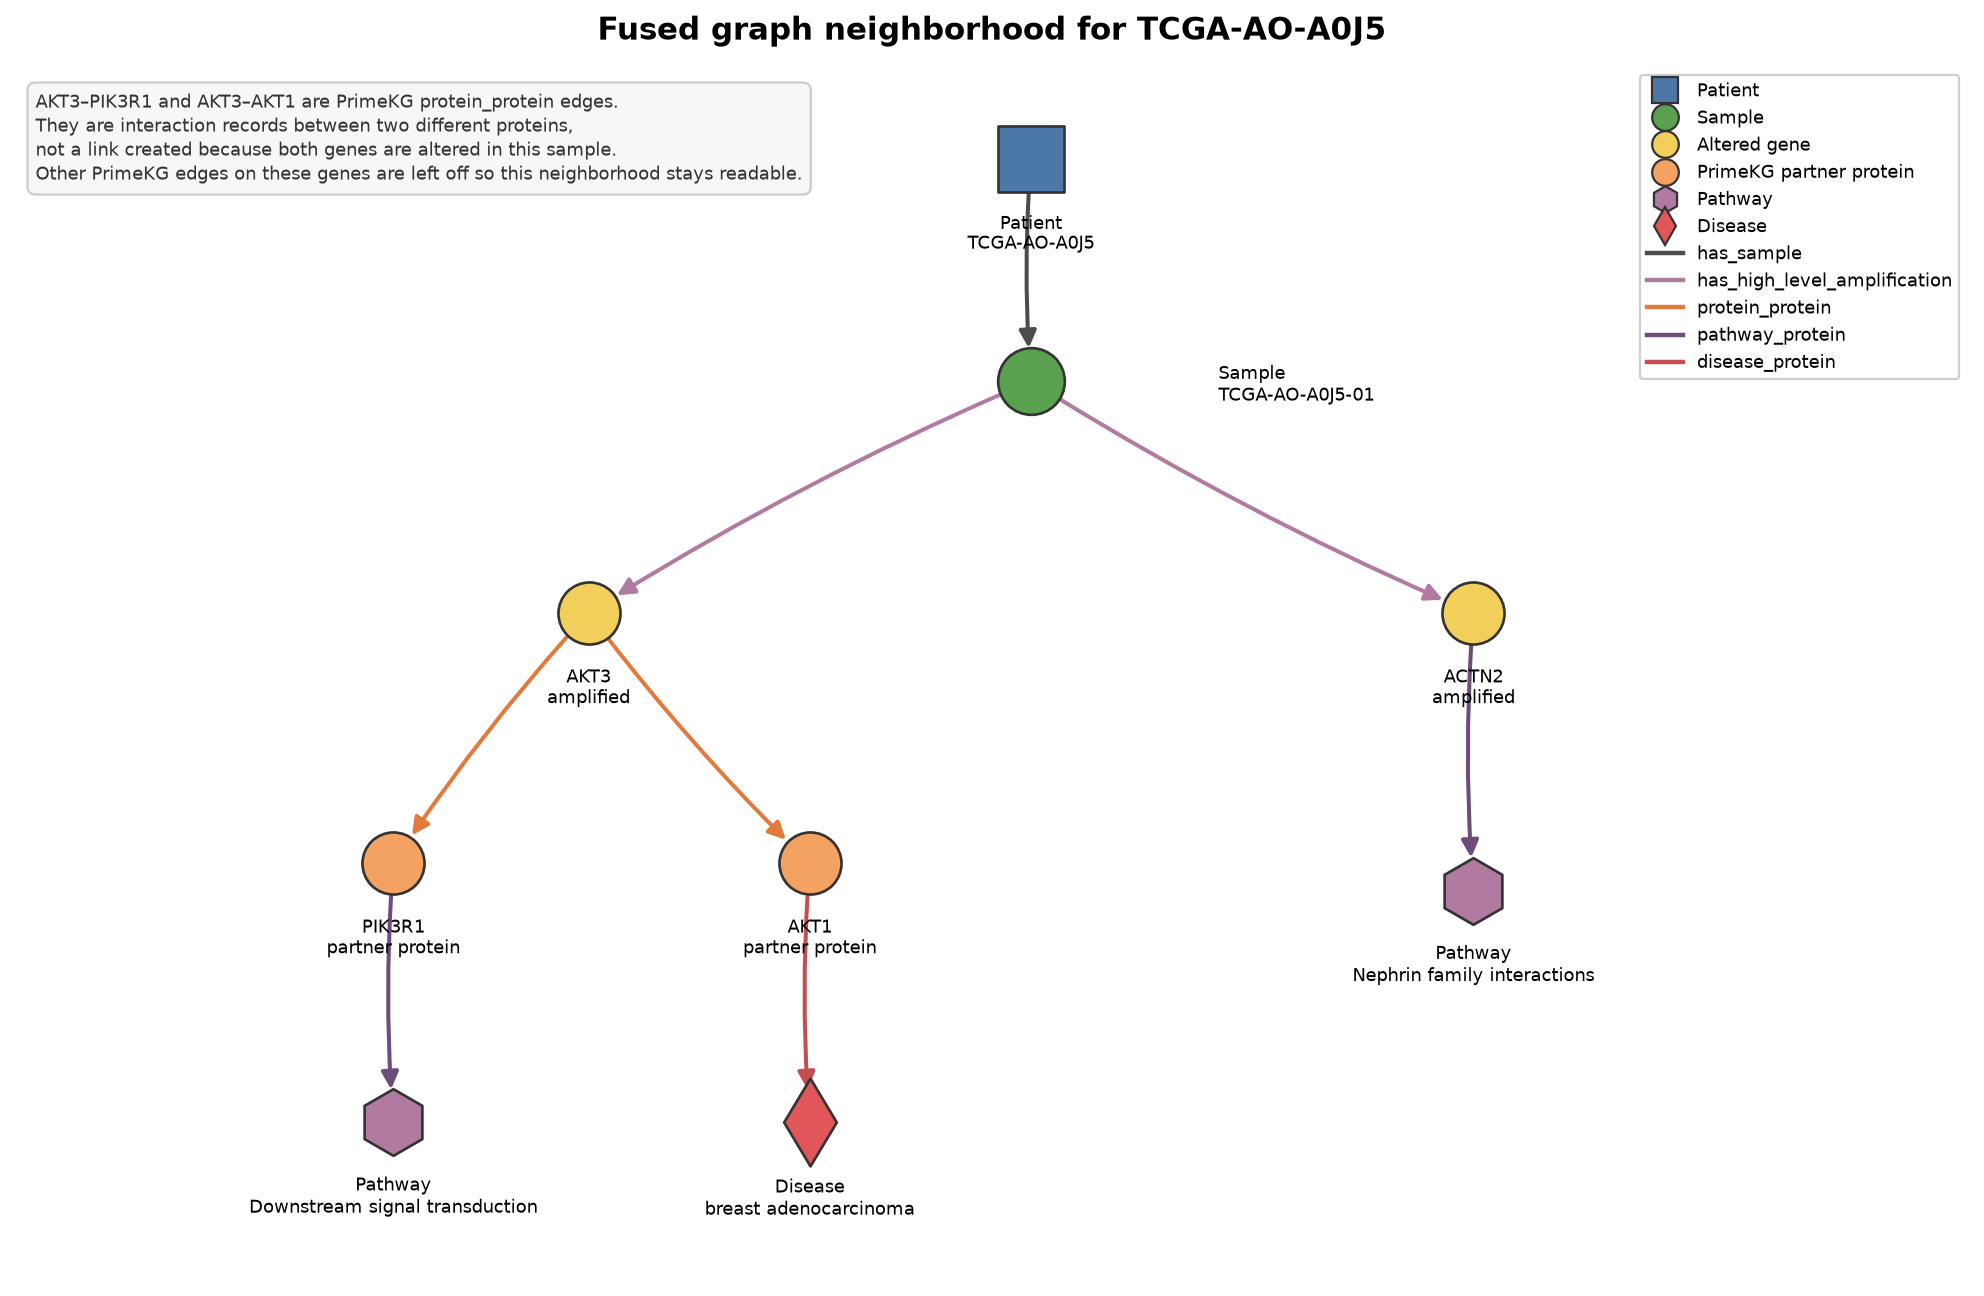
\includegraphics[width=0.55\textwidth]{fig_fused_graph.png}
  \caption{Part of a fused graph: a patient's altered genes linked to PrimeKG proteins, pathways, and a breast-disease node.}
  \label{fig:fused}
\end{figure}

\section{Neural Part: Graph Neural Networks}
All GNNs share three message-passing layers of width 64, a readout over the patient and altered-gene nodes, and a
clinical shortcut. On the landmark endpoint they are trained with cross-entropy or a smooth C-index loss. On the full
follow-up they are trained with the Cox partial likelihood, as in DeepSurv \rc{deepsurv}. The best survival GNN
supplies a neural risk. GNNExplainer, run on the fold model that held the patient out, gives every edge of the
patient's graph an importance score.

\section{Symbolic Part: From IF--THEN Rules to Learned Logic}\label{sec:logic}
\paragraph{Baseline.} RuleKit LR-Rules over 188 readable predicates gives about 8 crisp rules per fold. Only 10\% of
them mention the knowledge graph, and none of them carry a weight.

\paragraph{Ground atoms.} All new reasoners read the same 422 facts about each patient. There are 26 clinical atoms
such as $\mathit{NStage}(p,\mathrm{N3})$, 57 genomic atoms such as $\mathit{Mutated}(p,\mathrm{TP53})$, and 339
knowledge-graph atoms such as
\[
  \mathit{Altered}(p,g) \wedge \mathit{InPathway}(g,\text{PI3K Cascade}),
\]
whose value is the number of the patient's altered genes in that pathway. Atoms are chosen by prevalence (3--90\% of
patients), never by outcome.

\paragraph{1. Survival Markov logic network.} Every formula has the form
$w_k: \mathit{Body}_k(p) \Rightarrow \mathit{Progress}(p)$. A body is one atom or a clinical $\times$ knowledge-graph
pair found on the training fold. A patient's risk is the weighted count of the formulas that hold for them:
\begin{equation}
  \eta(p) = \sum_k w_k \log\big(1 + n_k(p)\big),
\end{equation}
where $n_k(p)$ is the number of ways formula $k$ is true for patient $p$. The novelty is in how $w$ is learned. A
standard MLN would treat every patient who has not relapsed \emph{yet} as a non-progressor. We instead learn $w$ with
the Cox partial likelihood, which uses each patient's follow-up time correctly, plus an elastic-net penalty
\rc{coxnet}. The penalty sets the weight of useless formulas to exactly zero, which performs structure learning.

\paragraph{2. Survival PSL.} Truth values are soft. The program has a rule per fact (``fact $\Rightarrow$ high risk''
and ``fact $\Rightarrow$ low risk'') and a collective rule, $\mathit{Similar}(p,q) \wedge \mathit{HighRisk}(q)
\Rightarrow \mathit{HighRisk}(p)$, that links each patient to their ten most similar training patients. Censoring is
handled with soft targets: a patient censored at 20 months gets the Kaplan--Meier probability of progressing before 36
months, given that they were still progression-free at 20.

\paragraph{3. Reinforcement-learned rules.} A small recurrent network writes a rule one atom at a time (up to three
atoms) and is trained with REINFORCE \rc{reinforce}. Its reward measures \emph{stability}. The training fold is split
into two halves, and a rule is rewarded only if it separates fast from slow progressors in the same direction in both
halves. A rule is kept only if it also separates them on a further 30\% of the fold that the search never saw.

\paragraph{4. RL-structured survival MLN (the engine).} The rules that survive RL's filter are added to the MLN's
candidate formulas, and the survival MLN learns every weight. RL does the structure learning and the survival
likelihood does the weight learning. Reasoners within one standard error of the best mean C-index are treated as tied
\rc{cart}, and among them the one with the richest reasoning becomes the engine.

\section{Fusion, Model Choice, and Month of Progression}
The final risk comes from a Cox model on three inputs: the 19 clinical fields, the GNN risk, and the logic-engine
risk. It is compared with clinical-only Cox models and a random survival forest \rc{rsf}. Among the models tied with
the best, we choose the one that can explain its prediction.

Most patients never progress, so we estimate the month of progression \emph{given} that progression happens. A
log-logistic AFT model is fitted on the training-fold progressors and checked against the recorded months of held-out
progressors.

\section{Explanation Paths: 0.6 Neural + 0.4 Rule}
A candidate path is a real walk in the patient's fused graph: patient $\rightarrow$ sample $\rightarrow$ altered gene
$\rightarrow$ (partner protein) $\rightarrow$ pathway, drug, or breast disease. Its score combines the two halves of
the system:
\begin{equation}
  \text{score}(\text{path}) = 0.6 \times \text{neural} + 0.4 \times \text{rule}.
\end{equation}
\emph{Neural} is the percentile of the path's mean GNNExplainer edge importance. \emph{Rule} is the summed weight of
the engine's formulas that the path supports, scaled to the range 0 to 1. A formula counts when it holds for the
patient and mentions the path's end node, its altered gene, or a gene on the path. Its sign shows whether the evidence
points to faster or slower progression. A path is \emph{prominent} if its score is in the top 20\% of the cohort. A
report shows $K = \min(5, \text{prominent paths})$ paths and tops up to at least three.

\section{Patient Reports}
Reports are grouped by the recorded progression month: A ($\le$12 months, 32 patients), B (12--24, 30), C (24--36, 27),
D ($>$36, 56), and N (no progression recorded, 938). Each report is a two- to three-page PDF. It shows the
clinical record, the risk percentile and the chance of progression at 12, 24, 36, and 60 months, the estimated
progression month next to the recorded outcome, and the patient's survival curve. It then lists the top-$K$ paths, the
weighted formulas that fire for the patient, the molecular profile, and the most similar patients. Each group also has
a summary page.

% ===========================================================================
\chapter{Results and Analysis}\label{ch:results}
% ===========================================================================

\section{Setup}
All experiments ran on an 8-core laptop without a GPU, in Python with PyTorch Geometric \rc{pyg}, lifelines
\rc{lifelines}, scikit-survival \rc{sksurv}, and RuleKit. Every result comes from stratified five-fold
cross-validation with a fixed seed. Every prediction is \emph{out-of-fold}: it comes from models trained on the four
folds that exclude that patient. The full pipeline takes about 50 minutes, and the 1,083 reports take about 5 minutes.

\section{Graph Neural Networks: Accuracy Saturates}
Table~\ref{tab:gnn} summarises the GNN benchmark on the 36-month landmark. The clinical logistic regression is the
strongest model. GCN comes close, and the gene-only network is weakest. Relation-aware models, a C-index loss, and
graph structure learning \rc{gslsurvey}, which learns which PrimeKG edges to keep, all stayed within the fold-to-fold
noise. On an external microarray cohort (GSE2034 \rc{gse2034}) the graph models also did not beat a linear baseline.

\begin{table}[!htbp]
  \centering
  \small\setlength{\tabcolsep}{5pt}
  \caption{36-month progression (498 patients, 89 events), five-fold mean $\pm$ standard deviation. A random ranking
  has an AUPRC of 0.18.}
  \label{tab:gnn}
  \begin{tabular}{lcc}
    \toprule
    Model & AUROC & AUPRC \\
    \midrule
    Clinical logistic regression & $0.703 \pm 0.081$ & $0.463 \pm 0.133$ \\
    GCN & $0.680 \pm 0.076$ & $0.396 \pm 0.091$ \\
    GraphSAGE & $0.650 \pm 0.045$ & $0.379 \pm 0.091$ \\
    GATv2 & $0.631 \pm 0.046$ & $0.355 \pm 0.060$ \\
    MLP (clinical + gene list) & $0.562 \pm 0.098$ & $0.262 \pm 0.064$ \\
    \bottomrule
  \end{tabular}
\end{table}

\section{Symbolic Reasoners Compared}\label{sec:logicresults}
Table~\ref{tab:logic} and Figure~\ref{fig:logic} compare the four reasoners with RuleKit on the full follow-up.

\begin{table}[!htbp]
  \centering
  \small\setlength{\tabcolsep}{4pt}
  \caption{Symbolic reasoners: five-fold C-index, formulas kept per fold, and the share of formulas that use PrimeKG.}
  \label{tab:logic}
  \begin{tabular}{lccc}
    \toprule
    Reasoner & C-index & Formulas/fold & Use PrimeKG \\
    \midrule
    Survival MLN & $0.630 \pm 0.055$ & 32.8 & 63\% \\
    \textbf{RL-structured MLN (engine)} & $\mathbf{0.628 \pm 0.055}$ & 35.2 & \textbf{69\%} \\
    RuleKit IF--THEN rules (baseline) & $0.619 \pm 0.048$ & 7.8 & 10\% \\
    Survival PSL & $0.604 \pm 0.059$ & 40.0 & 63\% \\
    RL rules alone & $0.563 \pm 0.046$ & 25.6 & 91\% \\
    \bottomrule
  \end{tabular}
\end{table}

\begin{figure}[!htbp]
  \centering
  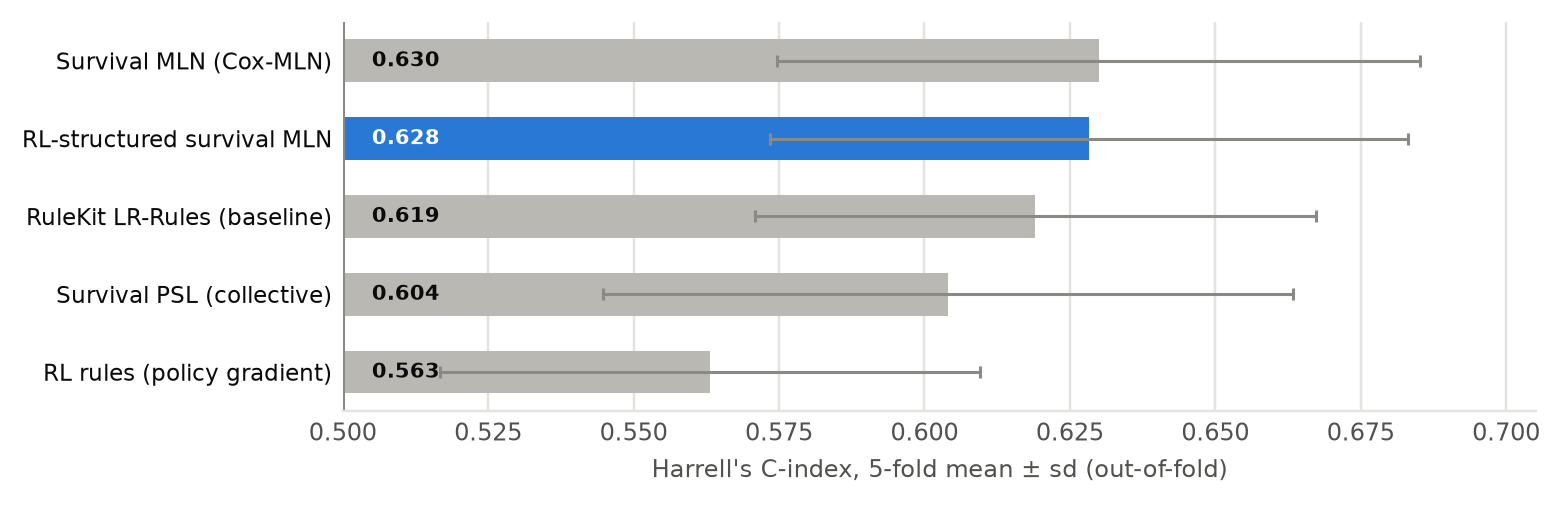
\includegraphics[width=0.7\textwidth]{fig_logic_comparison.png}
  \caption{Mean C-index of the symbolic reasoners over five folds. The chosen engine is highlighted.}
  \label{fig:logic}
\end{figure}

\paragraph{What the comparison shows.}
\begin{enumerate}
  \item \textbf{Accuracy is a tie.} Both MLN variants lead, but their gap over RuleKit (about 0.01) is smaller than the
        swing between folds (about 0.05). MLN, RL-structured MLN, and RuleKit are statistically tied, and the
        preference order selects the RL-structured MLN.
  \item \textbf{The reasoning is much richer.} The engine keeps about 35 weighted formulas per fold instead of 8 crisp
        rules, and 69\% of them reason over PrimeKG, about seven times RuleKit's share. Over the five folds it kept 176
        formulas: 51 single atoms, 81 mined clinical $\times$ PrimeKG pairs, and 44 multi-step formulas written by RL.
  \item \textbf{Collective reasoning found nothing.} PSL learned a weight of about 0.01 for ``similar patients have
        similar risk''. In this cohort, a patient's neighbours add no information beyond the patient's own facts.
  \item \textbf{RL alone overfits.} The agent tried 20,000--27,000 different rules per fold, so its best-looking rules
        are partly luck. RL works well as the formula \emph{proposer} for the MLN, where the survival likelihood decides
        which proposals count.
\end{enumerate}

\paragraph{Examples of learned formulas.} Clinical facts still carry the largest weights, for example
$\mathit{NStage}(p,\mathrm{N0}) \Rightarrow \mathit{Progress}(p)$ with weight $-0.30$ (slower progression). A mined
formula raises risk ($+0.15$, 43 patients):
\begin{multline*}
  \mathit{NStage}(p,\mathrm{N3}) \wedge \mathit{Altered}(p,g) \\ \wedge \mathit{LinkedTo}(g,\text{breast ductal adenocarcinoma}) \Rightarrow \mathit{Progress}(p).
\end{multline*}
An RL-proposed two-pathway formula is protective ($-0.14$, 93 patients; Figure~\ref{fig:rulekm}):
\begin{multline*}
  \mathit{Altered}(p,g) \wedge \mathit{InPathway}(g,\text{VEGFA-VEGFR2}) \\ \wedge \mathit{Altered}(p,g') \wedge \mathit{InPathway}(g',\text{Ion homeostasis}) \Rightarrow \mathit{Progress}(p).
\end{multline*}

\begin{figure}[!htbp]
  \centering
  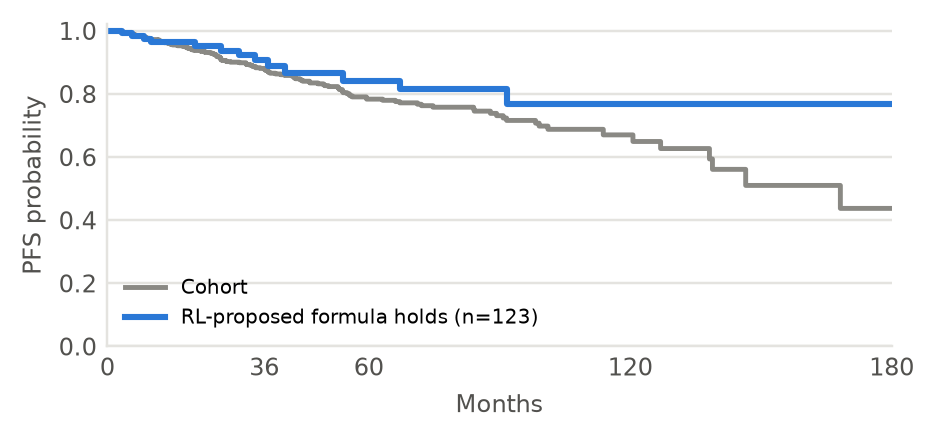
\includegraphics[width=0.48\textwidth]{fig_rule_km.png}
  \caption{Kaplan--Meier curve of the patients for whom the RL-proposed VEGFA-VEGFR2 / ion-homeostasis formula holds,
  against the whole cohort.}
  \label{fig:rulekm}
\end{figure}

\section{The Best Survival Model}
Table~\ref{tab:ns} compares the main models on the full follow-up. The best mean C-index is 0.675 (clinical Cox), with
one standard error of 0.016. Every model above 0.659 is statistically tied with it. Among the tied models we chose the
\textbf{neuro-symbolic Cox model} (0.664) because it is the only one whose prediction can be explained with paths and
formulas.

\begin{table}[!htbp]
  \centering
  \small\setlength{\tabcolsep}{4pt}
  \caption{Full follow-up (1,083 patients, 145 events): five-fold C-index and integrated Brier score to 120 months
  (IBS, lower is better).}
  \label{tab:ns}
  \begin{tabular}{lcc}
    \toprule
    Model & C-index & IBS \\
    \midrule
    Clinical Cox (19 fields) & $0.675 \pm 0.035$ & 0.134 \\
    \textbf{Neuro-symbolic Cox} (clinical + GNN + logic) & $\mathbf{0.664 \pm 0.021}$ & 0.134 \\
    GNN + logic, no clinical & $0.642 \pm 0.056$ & 0.139 \\
    RL-structured MLN alone & $0.628 \pm 0.055$ & -- \\
    Best GNN (GraphSAGE, C-index loss) & $0.622 \pm 0.067$ & -- \\
    Random survival forest & $0.554 \pm 0.023$ & 0.145 \\
    \bottomrule
  \end{tabular}
\end{table}

Two findings matter. First, every model family (GNN, logic, forest, and Cox) stops near a C-index of 0.67. With 145
events, stage, nodal status, age, and subtype carry most of the signal. Second, without clinical inputs the GNN and
logic risks together reach 0.642, better than either alone, but once the clinical fields are present they add no
independent information. The neuro-symbolic layer therefore adds \emph{explanation, not accuracy}. We state this
plainly in the report and in every patient report.

\section{Month of Progression}
On the 145 held-out progressors, the log-logistic AFT model is within 12 months of the recorded month for 48\% of
patients, against 37\% for a constant guess. It places 33\% of them in the correct 12-month window, against 19\% for the
constant guess and 25\% by chance. Its median error is 12.9 months (Figure~\ref{fig:timing}). Estimates are pulled
towards 15--45 months: very early progressions are overestimated and very late ones underestimated.

\begin{figure}[!htbp]
  \centering
  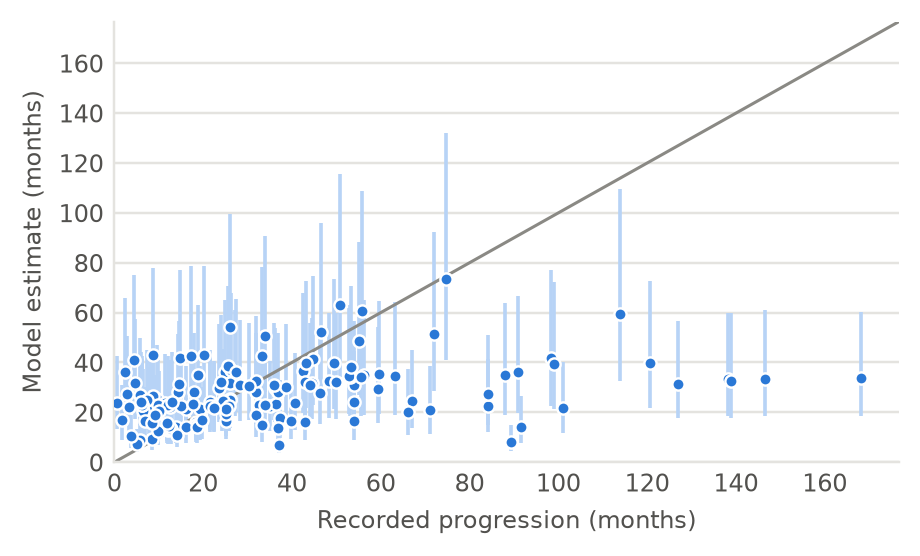
\includegraphics[width=0.45\textwidth]{fig_timing.png}
  \caption{Estimated against recorded progression month for held-out progressors. The diagonal is perfect agreement.}
  \label{fig:timing}
\end{figure}

\section{Explanation Paths and Reports}
The system scored 59,598 candidate paths for 1,033 patients. The other 50 patients have no altered gene with a PrimeKG
link. The prominence cutoff is a score of 0.523. 35\% of the paths shown in reports are backed by at least one learned
formula, and a median of three formulas fires per patient. Figure~\ref{fig:paths} shows the top paths of patient
TCGA-BH-A1EV (group A, progression at 12.0 months). All four are backed by formulas that raise the hazard. The
strongest runs from the amplified gene NFASC to the pathway \emph{Neurofascin interactions}.
Figure~\ref{fig:report} shows the page of the patient's report that lists these paths and the formulas that fire.

\begin{figure}[!htbp]
  \centering
  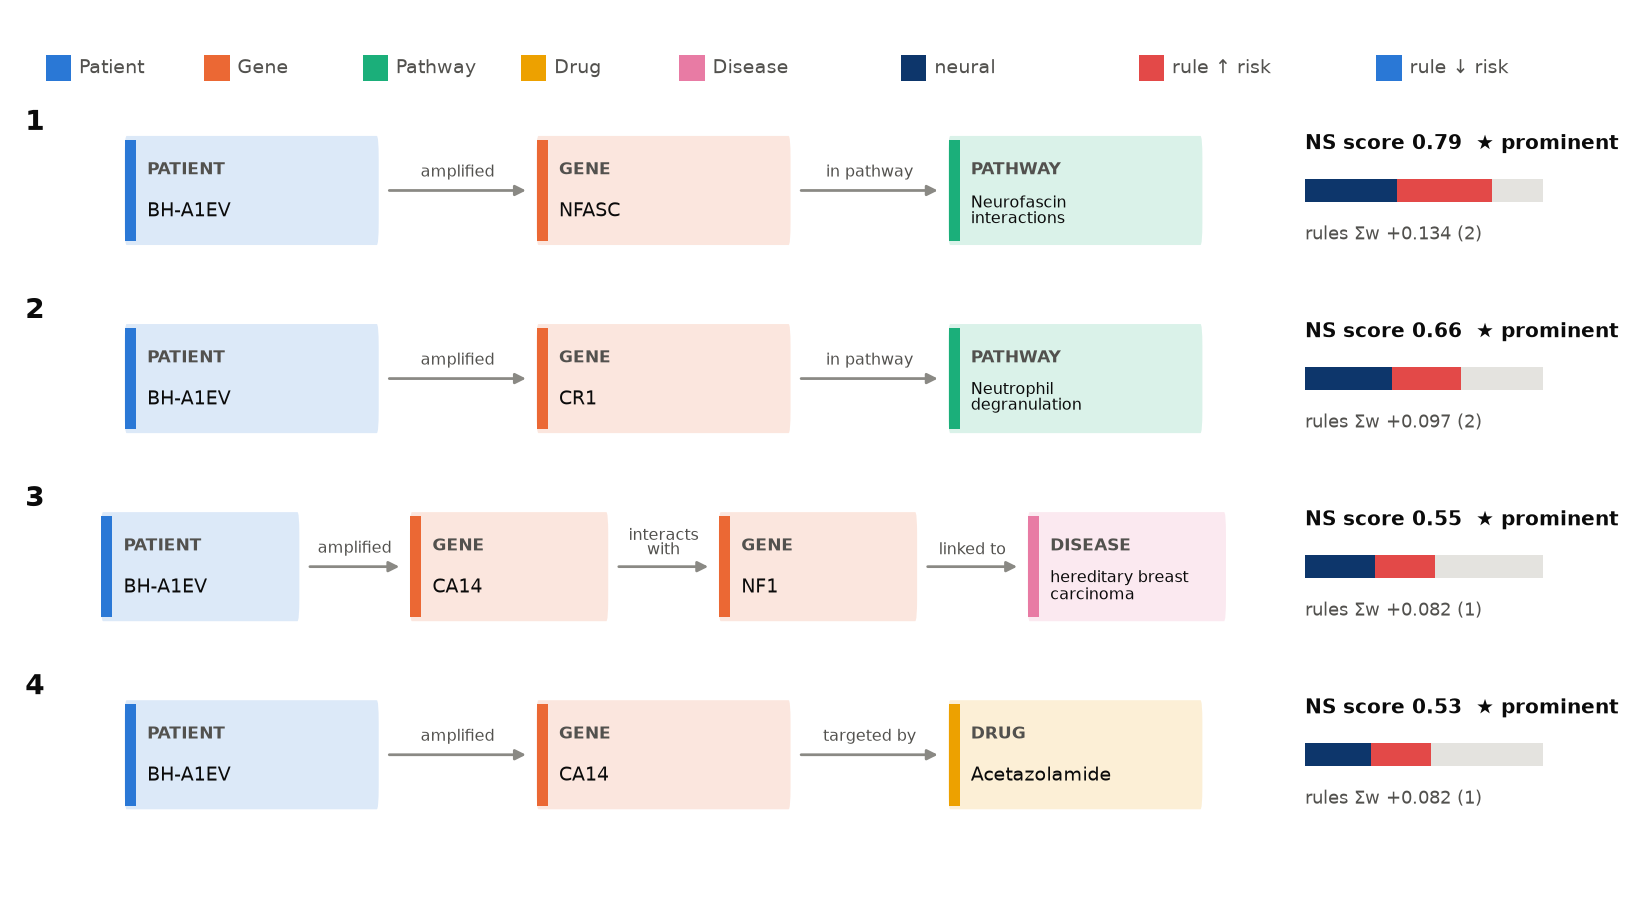
\includegraphics[width=0.85\textwidth]{fig_paths_example.png}
  \caption{Top-$K$ paths of TCGA-BH-A1EV. The bar on the right splits each score into its neural part (navy) and its
  rule part (red: the formulas raise the hazard).}
  \label{fig:paths}
\end{figure}

\begin{figure}[!htbp]
  \centering
  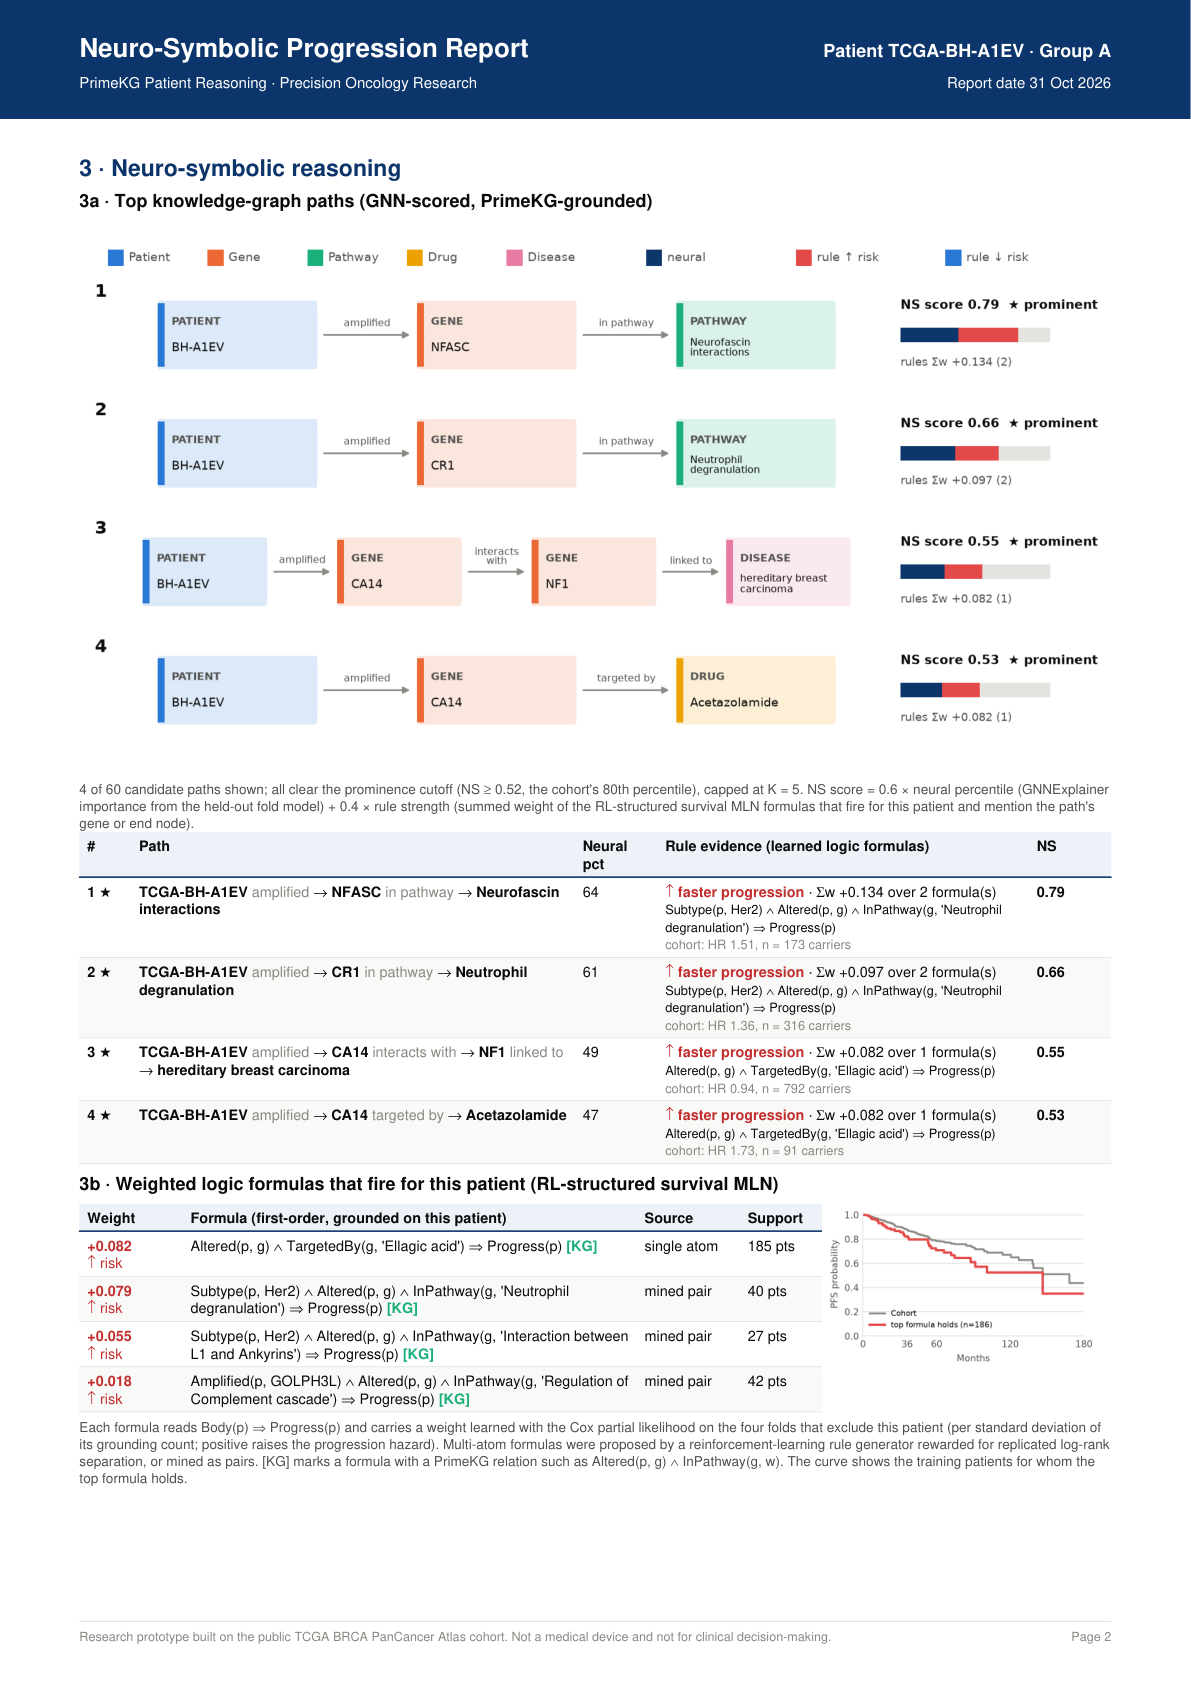
\includegraphics[width=0.5\textwidth]{fig_report_p2.png}
  \caption{Page 2 of the report of TCGA-BH-A1EV: top-$K$ knowledge-graph paths and the weighted logic formulas that fire.}
  \label{fig:report}
\end{figure}

% ===========================================================================
\chapter{Conclusion and Future Work}\label{ch:conclusion}
% ===========================================================================

\section{Conclusion}
We built a pipeline from raw TCGA tables to patient knowledge graphs fused with PrimeKG and benchmarked graph neural
networks on them. We then turned the system into a neuro-symbolic progression model with a report for every patient.
Following our supervisor's suggestion, we replaced IF--THEN rule induction with learned logic and compared Markov
logic, probabilistic soft logic, and reinforcement learning. The chosen engine is a survival Markov logic network: its
formulas are proposed by a reinforcement-learning agent and weighted with the Cox likelihood.

The engine matches the accuracy of the old rules and says far more. It keeps about four times as many formulas, they
carry weights, and 69\% of them reason over PrimeKG instead of 10\%. These formulas now drive the 0.4 rule part of
every explanation path. The fused model is tied with the best clinical model (C-index 0.664 against 0.675), and every
prediction is out-of-fold and leakage-checked. On this cohort, knowledge-graph reasoning adds explanation rather than
accuracy, and the system is designed around that finding.

\section{Limitations}
\begin{itemize}
  \item Accuracy saturates at a C-index of about 0.67 with 145 events.
  \item The month estimate is coarse, and late progressions are hard to place.
  \item Paths show what the model relied on. They are not causal claims, and PrimeKG drug links are not treatment advice.
  \item The work uses one cohort and one random seed, and the reports have not been validated externally.
\end{itemize}

\section{Future Work}
\begin{itemize}
  \item Let the RL agent walk multi-step PrimeKG relation paths and train it jointly with the MLN weights.
  \item Add expression and methylation data, and use pretrained knowledge-graph embeddings.
  \item Validate the model and the reports on an external cohort such as METABRIC.
  \item Ask oncologists to rate how useful and correct the reports are.
\end{itemize}

\noindent The code, the commands that reproduce every result, and two executed notebooks are in the project
repository: \path{notebooks/neurosymbolic_patient_reports.ipynb} walks through the whole system, and
\path{notebooks/symbolic_reasoning_novelty.ipynb} explains the logic reasoners and the novelty points.

% ===========================================================================
\renewcommand{\baselinestretch}{1.0}\normalsize
\chapter*{References}
\addcontentsline{toc}{chapter}{References}
\renewcommand{\labelenumi}{[\arabic{enumi}]}
\begin{enumerate}\setlength{\itemsep}{1pt}
\footnotesize
\item\label{ref:globocan} H.~Sung, J.~Ferlay, R.~L. Siegel, et al. Global cancer statistics 2020: GLOBOCAN estimates of incidence and mortality worldwide for 36 cancers in 185 countries. \emph{CA: A Cancer Journal for Clinicians}, 71(3):209--249, 2021.
\item\label{ref:pam50} J.~S. Parker, M.~Mullins, M.~C.~U. Cheang, et al. Supervised risk predictor of breast cancer based on intrinsic subtypes. \emph{Journal of Clinical Oncology}, 27(8):1160--1167, 2009.
\item\label{ref:primekg} P.~Chandak, K.~Huang, and M.~Zitnik. Building a knowledge graph to enable precision medicine. \emph{Scientific Data}, 10:67, 2023.
\item\label{ref:neurosymbolic} A.~d'Avila Garcez and L.~C. Lamb. Neurosymbolic AI: the 3rd wave. \emph{Artificial Intelligence Review}, 56:12387--12406, 2023.
\item\label{ref:hoadley} K.~A. Hoadley, C.~Yau, T.~Hinoue, et al. Cell-of-origin patterns dominate the molecular classification of 10,000 tumors from 33 types of cancer. \emph{Cell}, 173(2):291--304, 2018.
\item\label{ref:cbioportal} E.~Cerami, J.~Gao, U.~Dogrusoz, et al. The cBio cancer genomics portal: an open platform for exploring multidimensional cancer genomics data. \emph{Cancer Discovery}, 2(5):401--404, 2012.
\item\label{ref:tcgacdr} J.~Liu, T.~Lichtenberg, K.~A. Hoadley, et al. An integrated TCGA pan-cancer clinical data resource to drive high-quality survival outcome analytics. \emph{Cell}, 173(2):400--416, 2018.
\item\label{ref:gcn} T.~N. Kipf and M.~Welling. Semi-supervised classification with graph convolutional networks. In \emph{ICLR}, 2017.
\item\label{ref:graphsage} W.~L. Hamilton, R.~Ying, and J.~Leskovec. Inductive representation learning on large graphs. In \emph{NeurIPS}, 2017.
\item\label{ref:gatv2} S.~Brody, U.~Alon, and E.~Yahav. How attentive are graph attention networks? In \emph{ICLR}, 2022.
\item\label{ref:rgcn} M.~Schlichtkrull, T.~N. Kipf, P.~Bloem, R.~van den Berg, I.~Titov, and M.~Welling. Modeling relational data with graph convolutional networks. In \emph{ESWC}, pages 593--607, 2018.
\item\label{ref:gnnexplainer} R.~Ying, D.~Bourgeois, J.~You, M.~Zitnik, and J.~Leskovec. GNNExplainer: Generating explanations for graph neural networks. In \emph{NeurIPS}, 2019.
\item\label{ref:km} E.~L. Kaplan and P.~Meier. Nonparametric estimation from incomplete observations. \emph{Journal of the American Statistical Association}, 53(282):457--481, 1958.
\item\label{ref:logrank} N.~Mantel. Evaluation of survival data and two new rank order statistics arising in its consideration. \emph{Cancer Chemotherapy Reports}, 50(3):163--170, 1966.
\item\label{ref:cox} D.~R. Cox. Regression models and life-tables. \emph{Journal of the Royal Statistical Society: Series B}, 34(2):187--220, 1972.
\item\label{ref:aft} L.~J. Wei. The accelerated failure time model: a useful alternative to the Cox regression model in survival analysis. \emph{Statistics in Medicine}, 11(14--15):1871--1879, 1992.
\item\label{ref:harrell} F.~E. Harrell, R.~M. Califf, D.~B. Pryor, K.~L. Lee, and R.~A. Rosati. Evaluating the yield of medical tests. \emph{JAMA}, 247(18):2543--2546, 1982.
\item\label{ref:lrrules} \L.~Wr\'obel, A.~Gudy\'s, and M.~Sikora. Learning rule sets from survival data. \emph{BMC Bioinformatics}, 18:285, 2017.
\item\label{ref:rulekit} A.~Gudy\'s, M.~Sikora, and \L.~Wr\'obel. RuleKit: A comprehensive suite for rule-based learning. \emph{Knowledge-Based Systems}, 194:105480, 2020.
\item\label{ref:mln} M.~Richardson and P.~Domingos. Markov logic networks. \emph{Machine Learning}, 62(1--2):107--136, 2006.
\item\label{ref:psl} S.~H. Bach, M.~Broecheler, B.~Huang, and L.~Getoor. Hinge-loss Markov random fields and probabilistic soft logic. \emph{Journal of Machine Learning Research}, 18(109):1--67, 2017.
\item\label{ref:reinforce} R.~J. Williams. Simple statistical gradient-following algorithms for connectionist reinforcement learning. \emph{Machine Learning}, 8(3--4):229--256, 1992.
\item\label{ref:deeppath} W.~Xiong, T.~Hoang, and W.~Y. Wang. DeepPath: A reinforcement learning method for knowledge graph reasoning. In \emph{EMNLP}, pages 564--573, 2017.
\item\label{ref:minerva} R.~Das, S.~Dhuliawala, M.~Zaheer, et al. Go for a walk and arrive at the answer: Reasoning over paths in knowledge bases using reinforcement learning. In \emph{ICLR}, 2018.
\item\label{ref:rnnlogic} M.~Qu, J.~Chen, L.-P. Xhonneux, Y.~Bengio, and J.~Tang. RNNLogic: Learning logic rules for reasoning on knowledge graphs. In \emph{ICLR}, 2021.
\item\label{ref:deepsurv} J.~L. Katzman, U.~Shaham, A.~Cloninger, J.~Bates, T.~Jiang, and Y.~Kluger. DeepSurv: personalized treatment recommender system using a Cox proportional hazards deep neural network. \emph{BMC Medical Research Methodology}, 18:24, 2018.
\item\label{ref:coxnet} N.~Simon, J.~Friedman, T.~Hastie, and R.~Tibshirani. Regularization paths for Cox's proportional hazards model via coordinate descent. \emph{Journal of Statistical Software}, 39(5):1--13, 2011.
\item\label{ref:cart} L.~Breiman, J.~H. Friedman, R.~A. Olshen, and C.~J. Stone. \emph{Classification and Regression Trees}. Wadsworth, 1984.
\item\label{ref:rsf} H.~Ishwaran, U.~B. Kogalur, E.~H. Blackstone, and M.~S. Lauer. Random survival forests. \emph{The Annals of Applied Statistics}, 2(3):841--860, 2008.
\item\label{ref:pyg} M.~Fey and J.~E. Lenssen. Fast graph representation learning with PyTorch Geometric. In \emph{ICLR Workshop on Representation Learning on Graphs and Manifolds}, 2019.
\item\label{ref:lifelines} C.~Davidson-Pilon. lifelines: survival analysis in Python. \emph{Journal of Open Source Software}, 4(40):1317, 2019.
\item\label{ref:sksurv} S.~P\"olsterl. scikit-survival: A library for time-to-event analysis built on top of scikit-learn. \emph{Journal of Machine Learning Research}, 21(212):1--6, 2020.
\item\label{ref:gslsurvey} Y.~Zhu, W.~Xu, J.~Zhang, et al. A survey on graph structure learning: Progress and opportunities. \emph{arXiv preprint arXiv:2103.03036}, 2021.
\item\label{ref:gse2034} Y.~Wang, J.~G.~M. Klijn, Y.~Zhang, et al. Gene-expression profiles to predict distant metastasis of lymph-node-negative primary breast cancer. \emph{The Lancet}, 365(9460):671--679, 2005.
\end{enumerate}

\end{document}
